\subsection{MF POS short sequences \label{sec:pos_short_sequences}}

Another possible stylistic aspect that can be detected from a text using the MFW approach is to consider the sentence constructions.
This can be solved by creating short sequences ($n$-grams) of POS tags.
In this case, each POS is considered as a character in the letters $n$-grams in definition, this type of $n$-grams is also known as w-shingling.
For example, the sentence : \textit{"The cat eat a fish"} has the following POS tag \textit{"Article Noun Verb Article Noun"} which correspond to the following 3-grams of POS : \textit{"Article Noun Verb"} / \textit{"Noun Verb Article"} / \textit{"Verb Article Noun"}.
In practice the POS is more detailed, for example instead of just considering \textit{eat} as a verb, a more detailed POS can be the verb and its tense \textit{Verb-SimplePresent}, the same goes for the other type of POS.

When using features vectors based on the MFW method, once each document is represented as a feature vector they can be compared using metric in Section~\ref{sec:vectors_distances}.

\subsubsection{Evaluation}

For this experiment, short combination of POS are used to detect the style of the author.
POS $1$-grams are discarded from the experiment (equivalent of the POS frequency) since previous studies showed that POS $1$-grams tends to produce worse results then POS $2$/$3$/$4$-grams~\cite{kocher_linking}.
The St-Jean dataset have for every word a POS tag, by using these POS tags and combining them using Definition~\ref{def:letters_n_grams} to create $n$-grams/w-shingling, a new text representation is obtained.
This representation can be related to the author style sentence structure.
As for previous methods, the rank list is computed by scoring every document pairs, using the feature vector created with the MFW POS $n$-grams.
The experiment is split in two parts, the first aim to select the most convincing size of POS $n$-grams and the size of the feature vector.
The second is to compare the different distance metrics.
Keep in mind, as for the previous experiment in two parts, this experimentation methodology ignore the strength and weakness of distance measure with regard to the dimensionality of the vectors.

\subsubsection{Evaluation first part}

In this experiment, only $2$-grams, $3$-grams, $4$-grams and the combination of the $2$-grams and $3$-grams denoted: $(2, 3)$-grams is used.
The distance metric used for this part is the smoothed Z-Score normalized Cosine distance.
For this representation no clear MFW vector size is advised (in this case POS $n$-grams are considered as words in the MFW definition), the size used is between 200 and 2000 with a step of 100.
Figure~\ref{fig:pos_ngrams} show the average precision on the rank list produced by using POS $n$-grams over the number of MFW.

The two following information can be intuitively observed on this plot:
\begin{itemize}
  \item
  A more complex POS $n$-grams require more MFW to achieve its maximal effectiveness.
  In the St-Jean corpus, a total of 26 different POS are used to describe every words in the corpus.
  Which correspond to $26^2 = 676$ possible unique POS $2$-grams sequences, to $26^3 = 17,576$ POS $3$-grams and $26^4 = 456,976$ POS $4$-grams, thus $2$-grams converges and not $3$/$4$-grams.
  \item
  Like other methods, if the MFW ceiling is too high, an overfitting to less important words is possible, thus reducing the average precision.
  In Figure~\ref{fig:pos_ngrams} the POS 2-grams clearly have a drop in average precision after $\sim 250$-MFW.
\end{itemize}

Using the smoothed Z-Score Cosine distance, the most appropriate configuration for the POS $n$-grams text representation on St-Jean seem to be $250$-MFW POS $2$-grams and $1000$-MFW POS $3$-grams.

\begin{figure}
  \centering
  \caption{Average precision over the MFW in the rank list generated using the Z-Score normalized Cosine distance on St-Jean POS n-grams text representation.}
  \label{fig:pos_ngrams}
  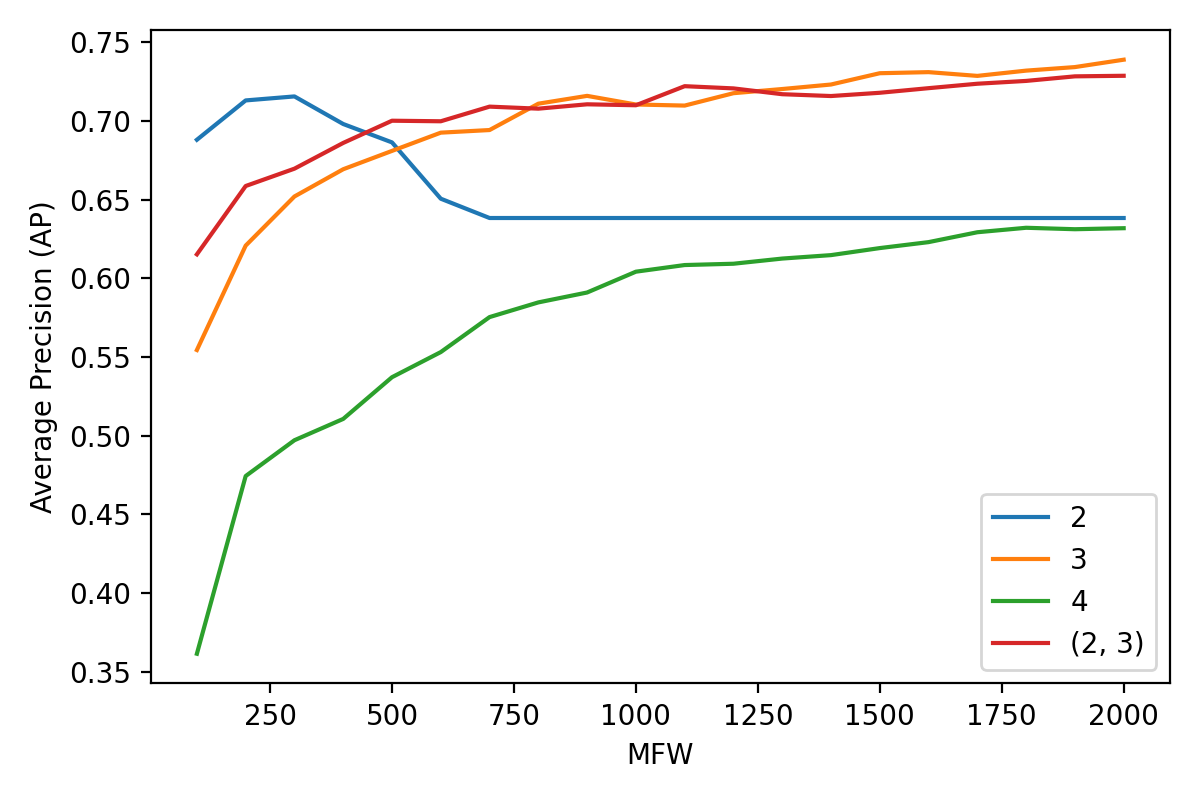
\includegraphics[width=\linewidth]{img/pos_ngrams.png}
\end{figure}

\subsubsection{Evaluation second part}

In this second part, the goal is to find the most appropriate distance metric for the POS $n$-grams text representation, with the configuration retained in the first part.
After running with these parameters on every proposed distance metrics, Table~\ref{tab:pos_ngrams} shows a resume of the experiment.

When considering POS $n$-grams as text representation on the St-Jean dataset, over all the best distance metrics are Manhattan, Matusita, Cosine distance.
The Clark distance, give overall the worse results, even though in other text representation, this metric was giving the best results.
Using an optimized distance metric can increase the average precision by up to $36$\% in average with this dataset and this text representation.

The retained configurations using the POS $n$-grams text representation is the $250$-MFW POS $2$-grams using the smoothed Z-Score Cosine Distance and $1000$-MFW POS $3$-grams using the smoothed Z-Scored Manhattan distance.

\begin{table}
  \centering
  \caption{Average precision for every distance metrics with the POS $n$-grams representation on St-Jean ($n$-grams/$n$-MFW)}
  \label{tab:pos_ngrams}
  \begin{tabular}{l c c c}
    \toprule
                    & \multicolumn{2}{c}{$n$-grams/$n$-MFW} \\
    Distance metric & $2$/$250$ & $3$/$1000$ \\
    \midrule
    Manhattan & 0.70 & \textbf{0.75} \\
    Tanimoto & 0.67 & 0.72 \\
    Euclidean & 0.69 & 0.72 \\
    Matusita & 0.70 & 0.73 \\
    Clark & 0.50 & 0.60 \\
    Cosine & \textbf{0.73} & 0.71 \\
    KLD & 0.68 & 0.70 \\
    JD & 0.69 & 0.73 \\
    \bottomrule
  \end{tabular}
\end{table}
